\documentclass[tikz,border=0pt]{standalone}
\usepackage[T1]{fontenc}
\usepackage{helvet}
\renewcommand{\familydefault}{\sfdefault}
% Reuse accepted label-free artwork through vector viewports; no pixel editing.
\usepackage{graphicx}
\usetikzlibrary{arrows.meta,calc}
\tikzset{flow/.style={-{Stealth[length=1.6mm,width=1.1mm]},line width=.5pt},
 every node/.style={font=\fontsize{9}{11}\selectfont,align=center,inner sep=1pt}}
% Arguments: source left/top/right/bottom pixels; destination left/bottom/width mm.
\newcommand{\artpiece}[7]{
 \pgfmathsetmacro{\pieceScale}{#7/((#3-#1)*.1)}
 \begin{scope}[shift={(#5,#6)},scale=\pieceScale,transform shape]
  \clip (0,0) rectangle ({(#3-#1)*.1},{(#4-#2)*.1});
  \node[anchor=south west,inner sep=0pt] at ({-#1*.1},{-(931-#4)*.1})
   {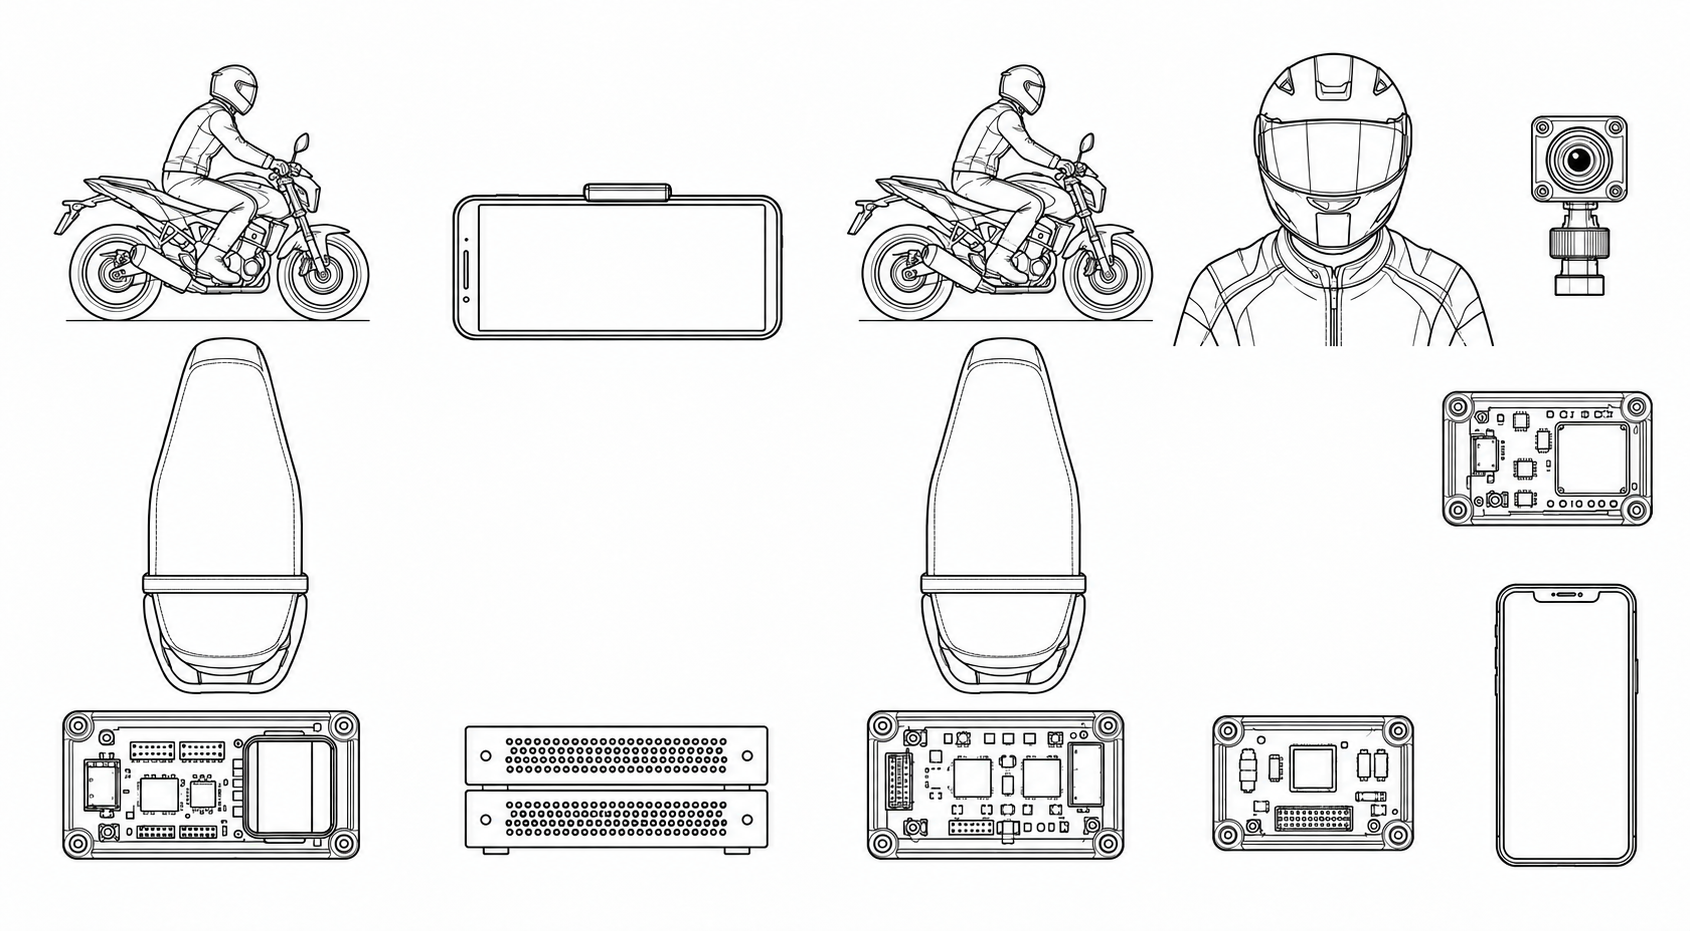
\includegraphics[width=169mm]{../reride/artwork-original.png}};
 \end{scope}}
\newcommand{\marker}[2]{
 \fill[white] (#1-2.4,#2-2.4) rectangle (#1+2.4,#2+2.4);
 \fill (#1-2,#2-2) rectangle (#1+2,#2+2);
 \fill[white] (#1-1.2,#2-1.2) rectangle (#1+1.2,#2+1.2);
 \fill (#1-1.2,#2-1.2) rectangle (#1,#2);
 \fill (#1,#2) rectangle (#1+1.2,#2+1.2);
}
\newcommand{\phoneglyph}[2]{
 \begin{scope}[shift={(#1,#2)}]
  \draw[densely dotted] (-8,0)--(8,0) (0,-13)--(0,13);
  \draw (0,10) .. controls (7,12) and (3,4) .. (7,-1)
    .. controls (11,-9) and (-4,-13) .. (-6,-7)
    .. controls (-9,0) and (-6,8) .. (0,10);
 \end{scope}}

\begin{document}
\begin{tikzpicture}[x=1mm,y=1mm,line width=.4pt,line cap=round,line join=round]
\path[use as bounding box] (0,0) rectangle (240,180);
\node at (120,171) {Posture data before, during and after motorcycle commuting};
\artpiece{35}{48}{380}{328}{8}{100}{65}
\node at (39,93) {Motorbike commute};
\artpiece{130}{330}{315}{700}{91}{106}{26}
% Two square FSRs, aligned left and right at the same fore/aft position.
\foreach \x in {100,108.3}{\draw[fill=white] (\x-1.8,128.5) rectangle (\x+1.8,132.1);}
\node at (104,164) {2 seat-pressure sensors};
\artpiece{55}{708}{370}{865}{78}{65}{53}
\node at (104,58) {Genuino};
\draw[flow] (104,106)--(104,92);
\artpiece{445}{178}{790}{345}{165}{116}{59}
\node at (195,152) {Live history + ride summary};
% Schematic UI glyphs, not measured pressure data.
\draw (172,128)--(178,128)--(178,136)--(185,136)--(185,125)
 --(192,125)--(192,132)--(200,132);
\draw (207,131) circle (5.5);
\draw (207,136.5)--(207,131)--(212,129);
\draw[flow] (131,78)--(145,78)--(145,131)--(165,131);
\node at (149,104) {Bluetooth};
\artpiece{455}{720}{775}{860}{168}{65}{53}
\node at (195,58) {Remote storage};
\draw[flow] (195,116)--(195,88.2);
\draw (8,47)--(232,47);
\node at (120,37) {Implemented interactive soft-and-hardware demonstration};
\node at (120,25) {2 FSRs; 1024 sensing levels; 4 feedback bands; data retained for later reflection};
\node at (120,12) {Platform capability demonstrated; posture accuracy and health outcomes not established};
\end{tikzpicture}
\end{document}
